\documentclass[lettersize,journal,onecolumn]{IEEEtran}
\usepackage[T1]{fontenc}
\usepackage{amsmath,amsfonts,amssymb}
\usepackage{array}
\usepackage{booktabs}
\usepackage{graphicx}
\usepackage{url}
\usepackage{cite}
\usepackage[hidelinks]{hyperref}
\graphicspath{{figures/}}
\hyphenation{Efficient-Net SIPaKMeD NHANES question-naire}

\renewcommand{\thefigure}{S\arabic{figure}}
\renewcommand{\thetable}{S\arabic{table}}
\renewcommand{\thesection}{S\arabic{section}}
\renewcommand{\topfraction}{0.95}
\renewcommand{\bottomfraction}{0.7}
\renewcommand{\textfraction}{0.05}
\renewcommand{\floatpagefraction}{0.85}
\setcounter{topnumber}{4}
\setcounter{bottomnumber}{3}
\setcounter{totalnumber}{6}
\raggedbottom
% float-only pages: pack from the top instead of distributing the slack between floats
\makeatletter
\setlength{\@fptop}{0pt}
\setlength{\@fpsep}{14pt}
\setlength{\@fpbot}{0pt plus 1fil}
\makeatother

\begin{document}

\title{Supplementary Material for\\ ``Fusing Unpaired Cytology and Questionnaire Experts for Cervical Screening: A Calibrated Rule and Its Region of Validity''}
\author{Author One, Author Two, Author Three, and Author Four}
\maketitle

\begin{abstract}
This supplement reports the material referenced from the main paper: the composition of the two data sets, the training behaviour and per-class performance of the cytology expert, the full model comparison and subgroup breakdown for the questionnaire expert, and the complete sweeps behind the region-of-validity analysis. Every number is produced by the same scripts as the main paper and is out of fold or out of sample in the same sense. Section numbering here is independent of the main text; notation and abbreviations follow it.
\end{abstract}

%% =====================================================================
\section{Data Sets}

\subsection{SIPaKMeD}
The cytology expert is trained on SIPaKMeD, which distributes 966 whole-field images together with 4,049 single cells cropped from those same fields, 5,015 images in all. Fig.~\ref{fig:scounts} gives the composition class by class and separates the two image types, which matters because the conventional random split of this data set puts cropped cells and their parent fields on opposite sides of the partition: 404 of the 414 cropped cells in the Protocol~A test set share a slide with a training image. Fig.~\ref{fig:ssamples} shows one representative example per class and image type. The visual distinction the expert has to make is between dyskeratotic and koilocytotic cells on one hand, which carry the nuclear enlargement, hyperchromasia and perinuclear haloes of the squamous intraepithelial lesion spectrum, and metaplastic, parabasal and superficial--intermediate cells on the other, which are benign or normal. Classes are nearly balanced, ratio 1.19, and 41.8\% of images are abnormal; that figure is the prior the network learns and the quantity the fusion rule removes before using its output.

\begin{figure}[!htbp]
\centering
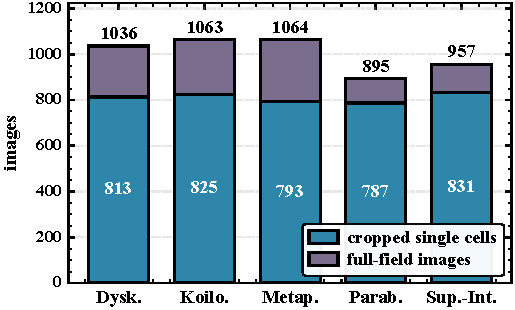
\includegraphics[width=3.45in]{img_dataset_counts}
\caption{Composition of SIPaKMeD by class, separating whole-field images from the single cells cropped out of them.}
\label{fig:scounts}
\end{figure}

\begin{figure}[!htbp]
\centering
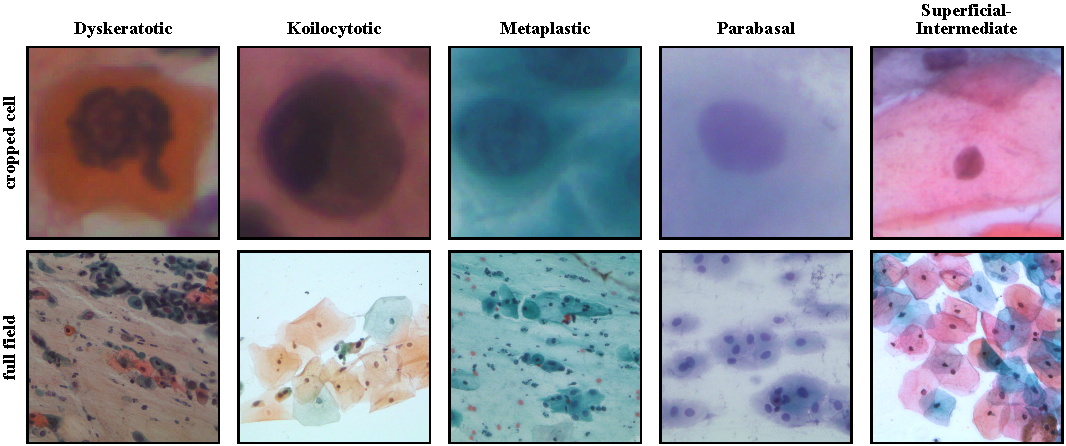
\includegraphics[width=\textwidth]{img_dataset_samples}
\caption{Representative examples of each SIPaKMeD class. Top row: whole-field images. Bottom row: cropped single cells. Dyskeratotic and koilocytotic cells are treated as abnormal throughout; metaplastic, parabasal and superficial--intermediate cells as normal.}
\label{fig:ssamples}
\end{figure}

\subsection{NHANES}
The questionnaire expert is trained on the 12,634 women aged 18--59 who provided a self-collected vaginal swab genotyped for HPV in the seven NHANES cycles from 2003--2004 to 2015--2016. Fig.~\ref{fig:scohort} shows the two gradients that carry most of the model's signal. Prevalence falls steeply with age, from 36\% at ages 18--24 to 17\% at 50--59, which reflects both the transience of most infections and the vaccination era reaching the youngest strata; and it rises with reported lifetime partners, from 9\% among women reporting at most one to 35\% among those reporting fifteen or more. Prevalence also falls across the survey period, from 29.1\% in 2005--2006 to 20.4\% in 2015--2016. That drift is exactly the prior-probability shift the re-anchoring step of the main paper is designed to absorb, and it is why the temporal experiment there loses calibration rather than discrimination.

\begin{figure}[!htbp]
\centering
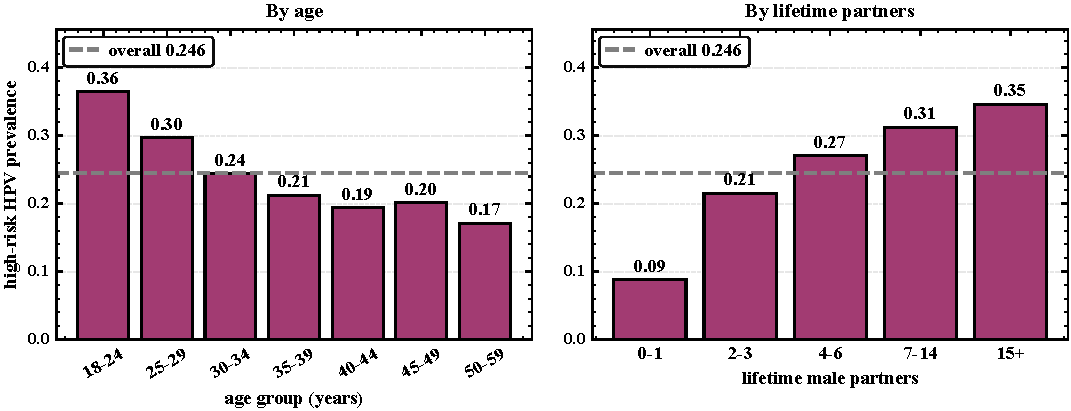
\includegraphics[width=\textwidth]{tab_cohort}
\caption{The NHANES analytic cohort. Left: high-risk HPV prevalence by age group. Right: prevalence by number of reported lifetime male partners. The dashed line is the cohort prevalence of 24.6\%.}
\label{fig:scohort}
\end{figure}

%% =====================================================================
\section{Cytology Expert}

\subsection{Training behaviour}
Fig.~\ref{fig:straining} shows the two-stage schedule. In stage~1 only the head is trained and validation accuracy plateaus near 0.90; unfreezing the backbone at the marked epoch produces the step to roughly 0.95, after which both curves flatten and early stopping on validation loss ends training. The student's distillation loss is shown on the same axes: it falls by two orders of magnitude within the first ten epochs, so almost all of the teacher's soft-label information is absorbed early, which is consistent with the ablation in the main paper finding little separation between distillation variants. The gap between training and validation accuracy stays under two points, so the augmentation and the frozen-then-fine-tuned schedule are doing their job.

\begin{figure}[!htbp]
\centering
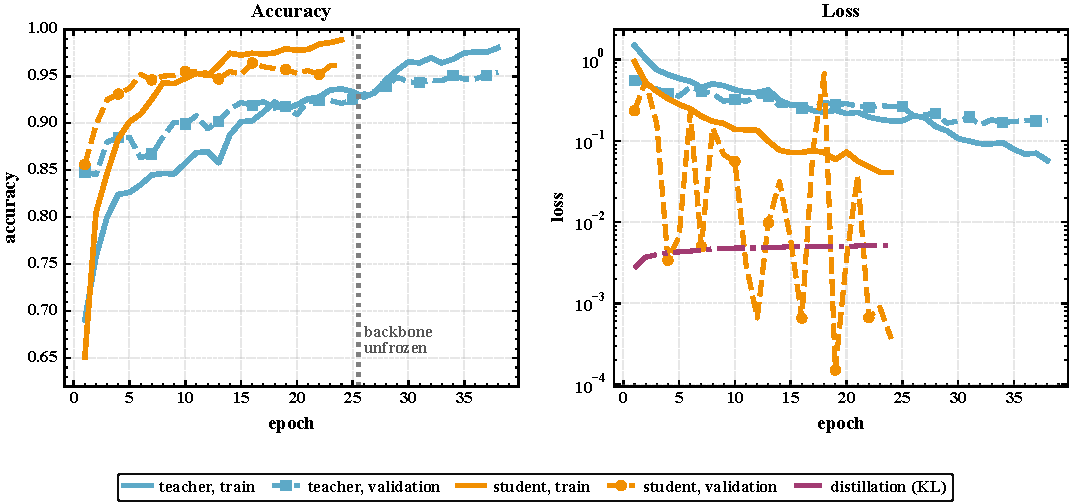
\includegraphics[width=\textwidth]{img_training}
\caption{Training behaviour. Left: accuracy for the teacher and the student, training and validation. Right: the corresponding losses, with the distillation term on a logarithmic axis. The vertical line marks the transition from head-only training to fine-tuning of the whole backbone.}
\label{fig:straining}
\end{figure}

\subsection{Per-class and threshold-free performance}
Table~\ref{tab:sperclass} gives precision, recall and F1 for every class on the fixed Protocol~A test set. No class falls below 0.92 on any measure for either network. The lowest recall belongs to metaplastic cells for the teacher (0.904), and inspection of the confusion matrix in the main paper shows those cells are lost to the abnormal classes rather than to the other normal ones, which is the conservative direction. Fig.~\ref{fig:sroc} gives the one-versus-rest ROC curves; every class exceeds 0.99 AUROC and the binary normal-versus-abnormal collapse exceeds 0.995 for both networks. Fig.~\ref{fig:sreliability} shows that both are close to the diagonal in distribution. It reports the calibration of the binary $P(\text{abnormal})$ that the fusion actually consumes, 0.017 for the teacher and 0.010 for the student, which is a different and easier quantity than the five-class expected calibration error of 0.024 and 0.020 given in the main paper; collapsing five classes to two averages out errors that are confined to the two abnormal classes. Either way the networks are well calibrated here, which is worth holding against their behaviour on an external collection, reported below and in the main paper.

\begin{figure}[!htbp]
\centering
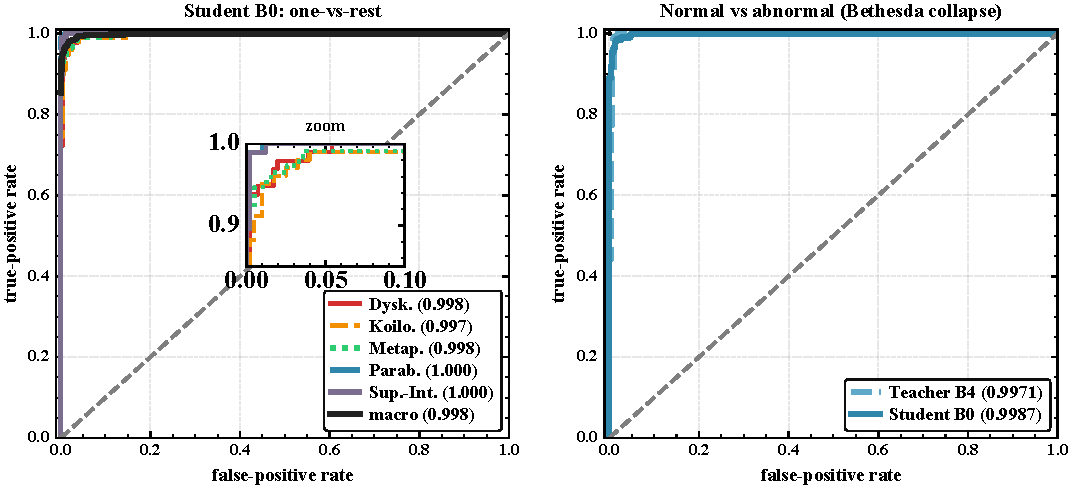
\includegraphics[width=\textwidth]{img_roc}
\caption{One-versus-rest ROC curves on the fixed Protocol~A test set, with the normal-versus-abnormal collapse on the right. The inset magnifies the top-left corner.}
\label{fig:sroc}
\end{figure}

\begin{table}[!htbp]
\caption{Per-Class Performance on the Fixed Protocol~A Test Set}
\label{tab:sperclass}
\centering\footnotesize
\begin{tabular}{@{}lccccccc@{}}
\toprule
Class & $n$ & \multicolumn{3}{c}{Teacher B4} & \multicolumn{3}{c}{Student B0} \\
\midrule
\cmidrule(lr){3-5}\cmidrule(l){6-8}
Metric & & Prec. & Rec. & F1 & Prec. & Rec. & F1 \\
Dyskeratotic & 97 & 0.940 & 0.969 & 0.954 & 0.931 & 0.969 & 0.949 \\
Koilocytotic & 102 & 0.907 & 0.951 & 0.928 & 0.959 & 0.922 & 0.940 \\
Metaplastic & 114 & 0.990 & 0.904 & 0.945 & 0.982 & 0.947 & 0.964 \\
Parabasal & 95 & 0.979 & 0.989 & 0.984 & 0.960 & 1.000 & 0.979 \\
Superficial-Intermediate & 96 & 0.990 & 1.000 & 0.995 & 0.990 & 0.990 & 0.990 \\
\bottomrule
\end{tabular}
\end{table}


\begin{figure}[!htbp]
\centering
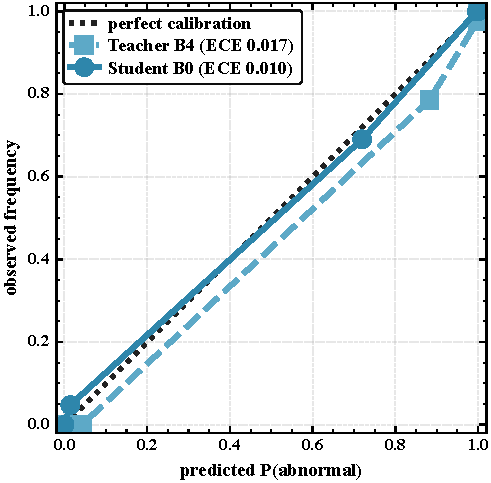
\includegraphics[width=3.45in]{img_reliability}
\caption{Reliability of the binary $P(\text{abnormal})$ that the fusion consumes, in equal-count bins on the Protocol~A test set. Both networks track the diagonal closely. These expected calibration errors are for the binary collapse and are therefore smaller than the five-class values quoted in the main paper.}
\label{fig:sreliability}
\end{figure}

\subsection{Slide-grouped protocol}
Fig.~\ref{fig:sgrouped} reports the protocol in which whole source slides are assigned to training, validation and test, so that no test cell shares a slide with any training cell. Per-class accuracy stays high and the ordering of the classes is unchanged, which is the evidence that the slide overlap present in the conventional split is not what produces the headline numbers. The two protocols nevertheless differ in composition as well as grouping -- Protocol~B uses cropped cells only, and its test set is smaller -- so the comparison is between two training runs and not a controlled equivalence test.

\begin{figure}[!htbp]
\centering
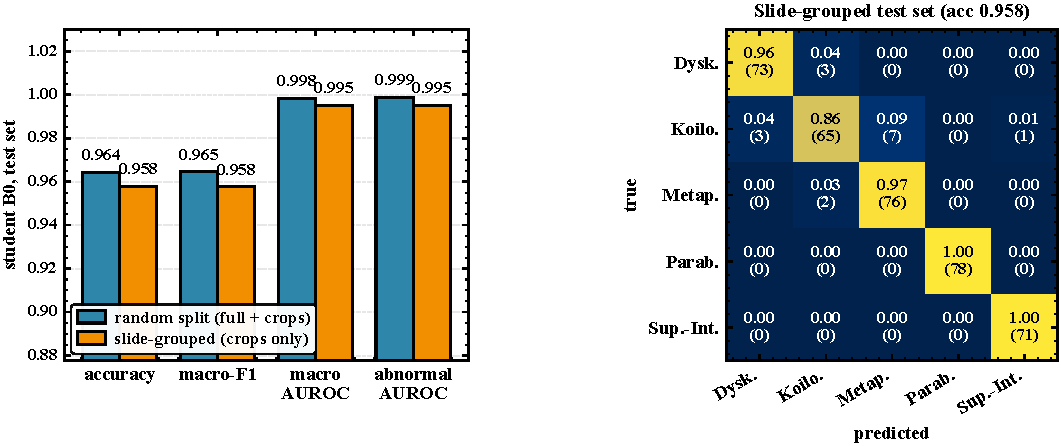
\includegraphics[width=\textwidth]{img_grouped}
\caption{The slide-grouped protocol. Left: per-class accuracy with whole slides held out. Right: the class composition of the resulting test set.}
\label{fig:sgrouped}
\end{figure}

\subsection{From cells to slides}
Table~\ref{tab:sslide} pools the held-out cells of each source slide into a slide score under four aggregators. All four exceed 0.997 AUROC and the mean and top-$k$ rules are indistinguishable. This is a change of unit rather than a change of difficulty: SIPaKMeD slides carry a single class, so a slide here is a homogeneous collection of cells, not a woman whose smear contains thousands of mostly normal cells among a few abnormal ones. The exercise is reported because it is the closest approach to the clinical unit the public data support, and because the gap between it and a real slide-level model is the clearest statement of what would be needed for patient-level calibration.

\begin{table}[!htbp]
\caption{Pooling Held-Out Cells Into Slide Scores}
\label{tab:sslide}
\centering\footnotesize
\begin{tabular}{@{}lccc@{}}
\toprule
Aggregator & AUROC & Average precision & Mean score \\
\midrule
mean & 0.9991 & 0.9991 & 0.465 \\
max & 0.9979 & 0.9976 & 0.498 \\
top3 & 0.9991 & 0.9991 & 0.476 \\
noisy-or & 0.9940 & 0.9930 & 0.501 \\
\midrule cell level (no pooling) & 0.9950 & --- & --- \\
\bottomrule
\end{tabular}
\\[2pt]\begin{minipage}{\textwidth}\scriptsize 97 slides (46 abnormal), 379 cells, median 3 cells per slide. The abnormal-slide prior is 0.474 against a cell-level prior of 0.401.\end{minipage}
\end{table}


\subsection{External behaviour, class by class}
Table~\ref{tab:sexternal} decomposes the external result by Herlev class. The pattern is not a uniform loss of accuracy. Normal superficial and intermediate cells are scored correctly, with mean abnormality 0.20 and 0.39 under the slide-grouped model; dysplastic and carcinoma \emph{in situ} cells are scored correctly too, between 0.61 and 0.85. The failure is confined to normal columnar cells, a type that does not exist in SIPaKMeD, which receive a mean score of 0.79 and a median of 0.979. The network has no representation for them and resolves the ambiguity towards abnormal. Excluding that one class raises external AUROC from 0.641 to 0.805.

\begin{table}[!htbp]
\caption{Mean Predicted Abnormality on Herlev, by Class}
\label{tab:sexternal}
\centering\footnotesize
\begin{tabular}{@{}llccc@{}}
\toprule
Herlev class & Mapped to & $n$ & Protocol A & Protocol B \\
\midrule
normal superficial & normal & 74 & 0.133 & 0.201 \\
normal intermediate & normal & 70 & 0.218 & 0.390 \\
normal columnar & normal & 98 & 0.470 & 0.788 \\
light dysplasia & abnormal & 182 & 0.625 & 0.757 \\
moderate dysplasia & abnormal & 146 & 0.529 & 0.700 \\
severe dysplasia & abnormal & 197 & 0.384 & 0.615 \\
carcinoma \emph{in situ} & abnormal & 150 & 0.517 & 0.847 \\
\bottomrule
\end{tabular}
\\[2pt]\begin{minipage}{\textwidth}\scriptsize Neither network ever saw a columnar cell. Both score that class as abnormal, which is what drives the drop in external AUROC; excluding it raises Protocol~B from 0.641 to 0.805.\end{minipage}
\end{table}


\subsection{What the network attends to}
Fig.~\ref{fig:sgradcam} shows Grad-CAM maps for correctly classified cells, computed on the pre-softmax class score because the gradients of a saturated softmax vanish. Attention concentrates on nuclei and perinuclear cytoplasm, which is where a cytologist looks. Two cautions apply. The final feature map is $12\times12$, so the localisation is coarse relative to a cell; and an attribution map shows where the gradient is large, not what decision rule the network applies. We report these as plausibility checks only.

\begin{figure}[!htbp]
\centering
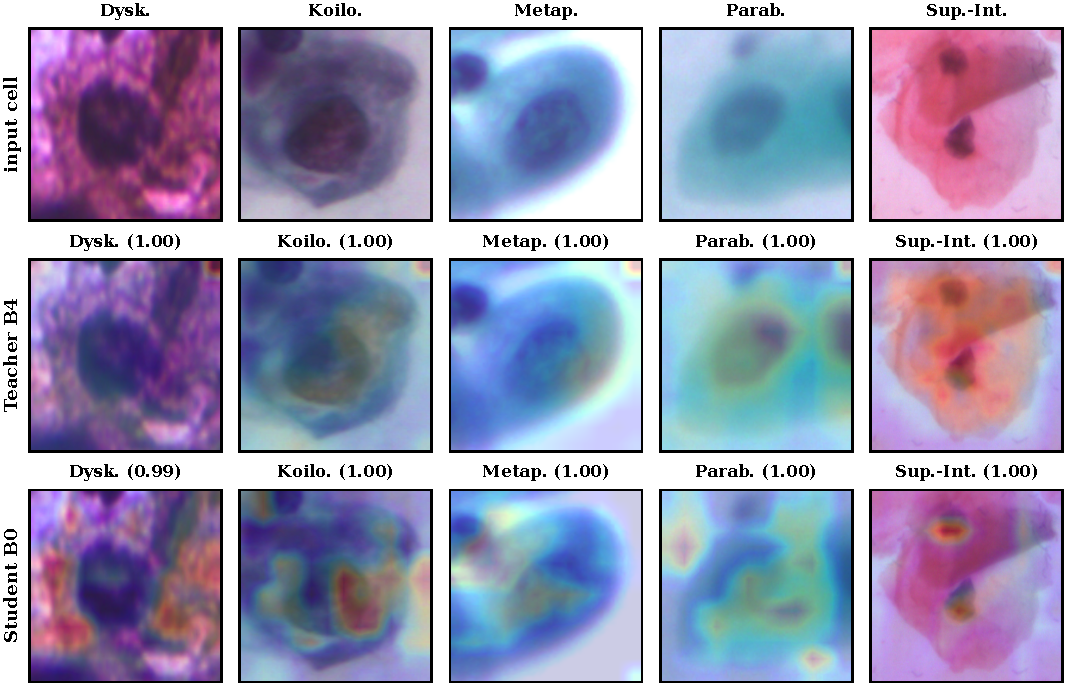
\includegraphics[width=\textwidth]{img_gradcam}
\caption{Grad-CAM maps for correctly classified cells. Top row: input. Middle: teacher. Bottom: student. Titles give the predicted class and its probability.}
\label{fig:sgradcam}
\end{figure}

%% =====================================================================
\section{Questionnaire Expert}

\subsection{Model comparison}
Table~\ref{tab:sfamilies} compares the six model families on identical folds, adding average precision and Brier score to the discrimination and calibration figures in the main paper. The ordering is the informative part: logistic regression, the three tree ensembles and the two boosting libraries all fall between 0.663 and 0.697 AUROC, a spread narrower than the fold-to-fold variation, while $k$-nearest neighbours is clearly worse at 0.615. Nothing in this problem rewards model capacity, which is what one expects when the inputs are two dozen self-reported risk factors and the outcome is a prevalent infection with a large stochastic component. Fig.~\ref{fig:smodels} shows the same comparison graphically. Because selecting the best of six families on the folds that also report the score is optimistic, the main paper uses a nested procedure; it chose logistic regression in all five outer folds and cost 0.003 AUROC.

\begin{table}[!htbp]
\caption{Questionnaire Model Families on Identical Folds}
\label{tab:sfamilies}
\centering\footnotesize
\begin{tabular}{@{}lcccc@{}}
\toprule
Model & AUROC & Avg.\ precision & Brier & ECE \\
\midrule
Logistic regression & 0.6972 & 0.4125 & 0.2204 & 0.222 \\
k-NN & 0.6151 & 0.3201 & 0.1998 & 0.120 \\
RandomForest & 0.6858 & 0.3958 & 0.1723 & 0.026 \\
ExtraTrees & 0.6632 & 0.3626 & 0.1822 & 0.059 \\
LightGBM & 0.6875 & 0.4102 & 0.1976 & 0.132 \\
XGBoost & 0.6856 & 0.4141 & 0.1995 & 0.141 \\
\midrule nested selection $+$ isotonic & 0.6945 & 0.4086 & 0.1699 & 0.022 \\
\bottomrule
\end{tabular}
\\[2pt]\begin{minipage}{\textwidth}\scriptsize All figures are out of fold with imputation, scaling and calibration fitted inside the training folds. The last row is the nested procedure reported in the main paper, which selected logistic regression in all five outer folds.\end{minipage}
\end{table}


\begin{figure}[!htbp]
\centering
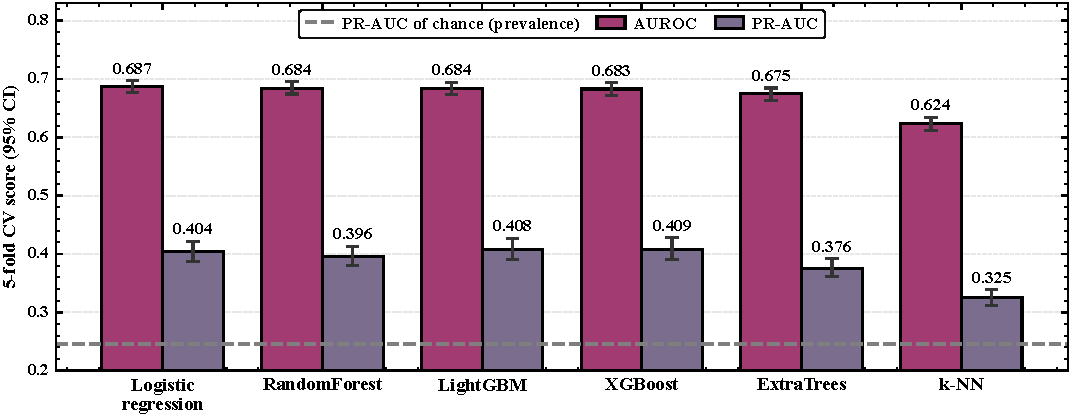
\includegraphics[width=\textwidth]{tab_models}
\caption{The six model families on identical folds, before nested selection. Differences among logistic regression and the ensembles are within the confidence intervals.}
\label{fig:smodels}
\end{figure}

\subsection{Discrimination and clinical usefulness}
Fig.~\ref{fig:stabcal} gives the reliability diagram of the calibrated expert alongside the raw class-weighted fit it replaces, and Fig.~\ref{fig:sroctab} its ROC curve. A questionnaire alone separates infected from uninfected women weakly, which is the reason the main paper uses it as a pre-test probability rather than as a decision rule: a weak but calibrated prior is useful in a Bayesian update even when it would be useless as a classifier. Fig.~\ref{fig:sdectab} gives the corresponding decision curve, which is positive over a band of threshold probabilities around the cohort prevalence and converges on the treat-all strategy at low thresholds, as any weak model must.

\begin{figure}[!htbp]
\centering
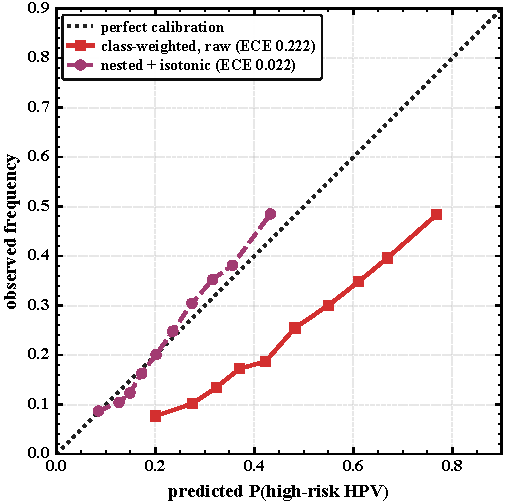
\includegraphics[width=3.45in]{tab_calibration}
\caption{Reliability of the questionnaire expert on out-of-fold predictions, before and after isotonic calibration. The calibrated model tracks observed frequency across the range in which it operates (ECE 0.022, slope 1.16); the uncalibrated class-weighted fit is systematically over-confident, because class weighting distorts the intercept.}
\label{fig:stabcal}
\end{figure}

\begin{figure}[!htbp]
\centering
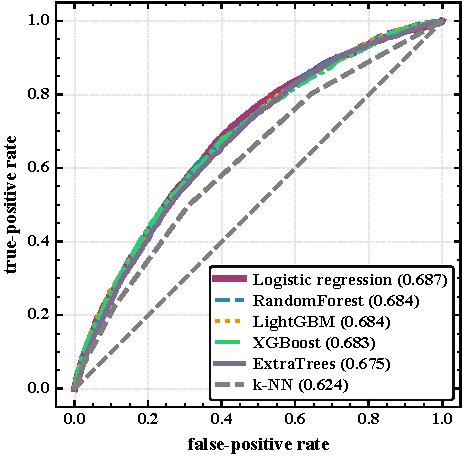
\includegraphics[width=3.45in]{tab_roc}
\caption{ROC curve of the calibrated questionnaire expert on out-of-fold predictions.}
\label{fig:sroctab}
\end{figure}

\begin{figure}[!htbp]
\centering
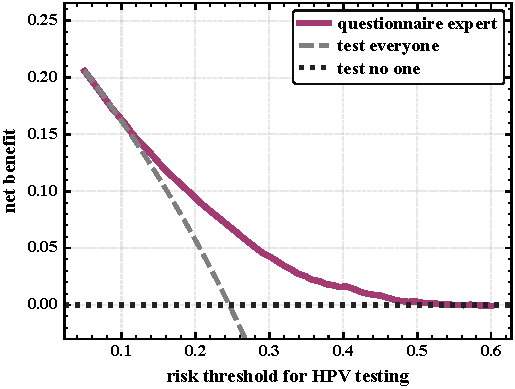
\includegraphics[width=3.45in]{tab_decision}
\caption{Decision-curve analysis of the questionnaire expert against treat-all and treat-none strategies.}
\label{fig:sdectab}
\end{figure}

\subsection{Subgroups, including survey cycle}
Table~\ref{tab:ssubgroups} extends the subgroup analysis of the main paper to every stratum with at least 200 women, including the seven survey cycles. Discrimination ranges from 0.637 to 0.725 and calibration error stays at or below 0.050 throughout. The two patterns worth noting are that the youngest stratum carries both the highest prevalence and the largest calibration error, and that performance by cycle is flat although prevalence across cycles is not, which is consistent with the model tracking individual risk factors rather than survey era.

\begin{table}[!htbp]
\caption{Questionnaire Expert by Subgroup, Including Survey Cycle}
\label{tab:ssubgroups}
\centering\footnotesize
\begin{tabular}{@{}lccccc@{}}
\toprule
Subgroup & $n$ & Prevalence & AUROC & Brier & ECE \\
\midrule
age 18-29 & 4093 & 0.341 & 0.683 & 0.207 & 0.050 \\
age 30-39 & 2907 & 0.228 & 0.682 & 0.164 & 0.030 \\
age 40-49 & 3029 & 0.197 & 0.640 & 0.153 & 0.015 \\
age 50-59 & 2605 & 0.171 & 0.638 & 0.137 & 0.006 \\
race/ethnicity: Mexican American & 2361 & 0.226 & 0.655 & 0.166 & 0.014 \\
race/ethnicity: Other Hispanic & 1227 & 0.236 & 0.637 & 0.172 & 0.015 \\
race/ethnicity: White & 4904 & 0.225 & 0.720 & 0.157 & 0.033 \\
race/ethnicity: Black & 2909 & 0.331 & 0.647 & 0.210 & 0.031 \\
race/ethnicity: Other & 1233 & 0.174 & 0.703 & 0.129 & 0.035 \\
cycle 2003-2004 & 1558 & 0.272 & 0.639 & 0.189 & 0.015 \\
cycle 2005-2006 & 1728 & 0.291 & 0.681 & 0.191 & 0.033 \\
cycle 2007-2008 & 1783 & 0.253 & 0.700 & 0.172 & 0.024 \\
cycle 2009-2010 & 1955 & 0.256 & 0.720 & 0.171 & 0.033 \\
cycle 2011-2012 & 1767 & 0.234 & 0.725 & 0.160 & 0.038 \\
cycle 2013-2014 & 1985 & 0.219 & 0.686 & 0.159 & 0.015 \\
cycle 2015-2016 & 1858 & 0.204 & 0.677 & 0.153 & 0.014 \\
\bottomrule
\end{tabular}
\\[2pt]\begin{minipage}{\textwidth}\scriptsize Groups with fewer than 200 women or a single outcome class are omitted. Discrimination varies by 0.09 AUROC and calibration error stays at or below 0.050 everywhere.\end{minipage}
\end{table}


\subsection{The full importance ranking}
Table~\ref{tab:simportance} gives the twenty most important inputs by permutation importance on held-out folds, without the exclusion applied in the main paper's figure. The top five are all missingness flags. This is a property of the estimator rather than of the data: the flags are near-collinear because all of them are driven by which cycle a woman was surveyed in, and the fitted model carries large offsetting coefficients on them, so permuting one destroys a cancellation the others depend on. The direct test is to remove all 27 flags, which costs 0.004 AUROC, against a model built on survey cycle alone which reaches only 0.539. We therefore report the substantive items in the main paper and give the raw ranking here for completeness.

\begin{table}[!htbp]
\caption{Permutation Importance of All Inputs, Top 20}
\label{tab:simportance}
\centering\footnotesize
\begin{tabular}{@{}lcccc@{}}
\toprule
Input & Missingness flag & AUROC drop & SD & Coefficient \\
\midrule
gonorrhea hx (asked?) & yes & +0.0914 & 0.0066 & +1.104 \\
herpes hx (asked?) & yes & +0.0492 & 0.0103 & -0.595 \\
chlamydia hx (asked?) & yes & +0.0411 & 0.0113 & -0.522 \\
ever oral man (asked?) & yes & +0.0394 & 0.0215 & -0.488 \\
age first oral (asked?) & yes & +0.0375 & 0.0177 & +0.314 \\
smoking status & no & +0.0312 & 0.0083 & +0.327 \\
ever sex (asked?) & yes & +0.0278 & 0.0239 & +0.322 \\
partners per active year & no & +0.0225 & 0.0081 & +0.347 \\
condomless year (asked?) & yes & +0.0209 & 0.0051 & -0.252 \\
ever oral man & no & +0.0202 & 0.0121 & +0.286 \\
smoked 100 (asked?) & yes & +0.0153 & 0.0094 & +0.218 \\
n vaginal partners life (asked?) & yes & +0.0144 & 0.0025 & -0.214 \\
n oral partners life (asked?) & yes & +0.0133 & 0.0165 & +0.134 \\
marital 1.0 & no & +0.0128 & 0.0159 & -0.174 \\
n partners year (asked?) & yes & +0.0120 & 0.0154 & +0.157 \\
smoked 100 & no & +0.0114 & 0.0053 & -0.188 \\
marital 5.0 & no & +0.0108 & 0.0070 & +0.150 \\
age & no & +0.0093 & 0.0048 & -0.154 \\
ever anal man (asked?) & yes & +0.0082 & 0.0080 & +0.150 \\
partners per active year (asked?) & yes & +0.0070 & 0.0063 & -0.097 \\
\bottomrule
\end{tabular}
\\[2pt]\begin{minipage}{\textwidth}\scriptsize Measured on held-out folds. Missingness flags record whether a question was asked at all. They head the ranking because they are collinear and carry large offsetting coefficients, so permuting one destroys a cancellation the others rely on; removing all 27 costs 0.0042 AUROC. The main paper's figure therefore shows the substantive items only.\end{minipage}
\end{table}


%% =====================================================================
\section{Fusion}

\subsection{Behaviour on a matched cohort}
Fig.~\ref{fig:sheadline} shows the ROC and reliability of every comparator on a matched cohort with an image expert of AUROC 0.90. The proposed rule and the paired-data oracle are visually indistinguishable in both panels, which is the verification that the implementation realises the Bayes rule its derivation predicts. The naive combinations rank slightly worse and are visibly miscalibrated, because averaging two probabilities that were calibrated at different priors produces a probability calibrated at neither.

\begin{figure}[!htbp]
\centering
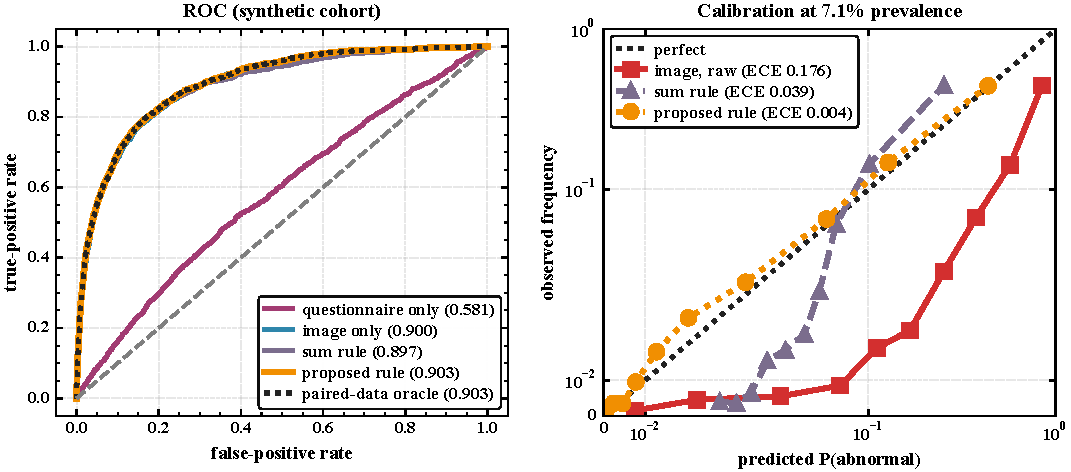
\includegraphics[width=\textwidth]{fus_headline_090}
\caption{ROC and reliability on a matched cohort with an image expert of AUROC 0.90.}
\label{fig:sheadline}
\end{figure}

\subsection{Getting the link wrong}
Fig.~\ref{fig:smisspec} varies the link used by the rule by up to a factor of ten in either direction from the value used to generate the cohort. Discrimination is almost unaffected, because a monotone reparametrisation of the pre-test odds barely changes the ranking, and calibration degrades gracefully rather than catastrophically. This is why the confidence interval on the estimated odds ratio, 17.5 to 18.3, is not a practical source of error: the rule would tolerate an interval two orders of magnitude wider than the one the data give.

\begin{figure}[!htbp]
\centering
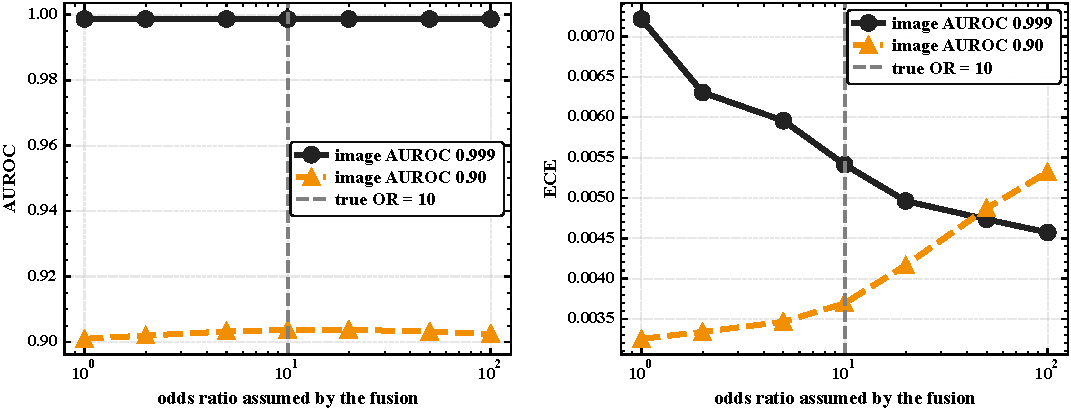
\includegraphics[width=\textwidth]{fus_misspec}
\caption{Misspecification of the epidemiological link. The cohort is generated at an odds ratio of 10 (dashed line) and the rule is told a value between a tenth and ten times that. Discrimination (top) is essentially flat; calibration error (bottom) rises smoothly and stays below 0.008 throughout.}
\label{fig:smisspec}
\end{figure}

\subsection{Every violation setting}
Table~\ref{tab:sviolations} gives all six violations at every strength, with all four comparators, rather than the representative rows selected for the main paper. Three observations are easier to see here than in the summary. Under V1 the naive mean degrades faster than the proposed rule even though the proposed rule is the one whose assumption is being broken, so the crossing point reported in the main paper is not an artefact of choosing a weak baseline. Under V2 the naive mean overtakes the proposed rule at every non-zero strength, because a direct questionnaire-to-cytology path makes the questionnaire more informative than the rule is willing to assume. And under V3 every method improves, because an infection-dependent shift of the image score adds information that all of them can use.

\begin{table}[!htbp]
\caption{Every Assumption-Violation Setting in Full}
\label{tab:sviolations}
\centering\scriptsize
\begin{tabular}{@{}lcccccc@{}}
\toprule
Setting & Image & Naive mean & Sum rule & Proposed & Oracle & ECE$_{\text{prop}}$ \\
\midrule
\multicolumn{7}{@{}l}{\emph{V1: residual dependence given the latent state}} \\
\quad $\rho$ $=$ 0 & 0.8947 & 0.8893 & 0.8911 & 0.8972 & 0.8969 & 0.010 \\
\quad $\rho$ $=$ 0.2 & 0.8978 & 0.8816 & 0.8885 & 0.8951 & 0.8979 & 0.010 \\
\quad $\rho$ $=$ 0.4 & 0.8980 & 0.8701 & 0.8821 & 0.8899 & 0.9037 & 0.009 \\
\quad $\rho$ $=$ 0.6 & 0.8982 & 0.8595 & 0.8764 & 0.8847 & 0.9217 & 0.008 \\
\quad $\rho$ $=$ 0.8 & 0.8984 & 0.8497 & 0.8712 & 0.8797 & 0.9587 & 0.008 \\
\multicolumn{7}{@{}l}{\emph{V2: direct questionnaire-to-cytology path}} \\
\quad $\gamma$ $=$ 0 & 0.8947 & 0.8893 & 0.8911 & 0.8972 & 0.8969 & 0.010 \\
\quad $\gamma$ $=$ 0.25 & 0.8953 & 0.8993 & 0.8979 & 0.9012 & 0.9027 & 0.012 \\
\quad $\gamma$ $=$ 0.5 & 0.8956 & 0.9075 & 0.9034 & 0.9044 & 0.9097 & 0.015 \\
\quad $\gamma$ $=$ 1 & 0.8940 & 0.9196 & 0.9115 & 0.9082 & 0.9245 & 0.024 \\
\multicolumn{7}{@{}l}{\emph{V3: infection affects the image at fixed cytology}} \\
\quad $\delta$ $=$ 0 & 0.8947 & 0.8893 & 0.8911 & 0.8972 & 0.8969 & 0.010 \\
\quad $\delta$ $=$ 0.1 & 0.9152 & 0.9064 & 0.9093 & 0.9160 & 0.9162 & 0.012 \\
\quad $\delta$ $=$ 0.2 & 0.9235 & 0.9141 & 0.9177 & 0.9233 & 0.9239 & 0.018 \\
\quad $\delta$ $=$ 0.4 & 0.9270 & 0.9156 & 0.9208 & 0.9250 & 0.9267 & 0.027 \\
\multicolumn{7}{@{}l}{\emph{V4: the link varies by subgroup}} \\
\quad spread $=$ 0 & 0.8947 & 0.8893 & 0.8911 & 0.8972 & 0.8969 & 0.010 \\
\quad spread $=$ 0.25 & 0.8944 & 0.8892 & 0.8910 & 0.8969 & 0.8966 & 0.010 \\
\quad spread $=$ 0.5 & 0.8937 & 0.8879 & 0.8897 & 0.8959 & 0.8957 & 0.011 \\
\multicolumn{7}{@{}l}{\emph{V5: an expert is miscalibrated by an unknown temperature}} \\
\quad questionnaire temperature 1 & 0.8947 & 0.8893 & 0.8911 & 0.8972 & 0.8969 & 0.010 \\
\quad questionnaire temperature 1.5 & 0.8947 & 0.8922 & 0.8919 & 0.8970 & 0.8969 & 0.010 \\
\quad questionnaire temperature 2 & 0.8947 & 0.8941 & 0.8928 & 0.8969 & 0.8969 & 0.010 \\
\quad image temperature 1.5 & 0.8947 & 0.8871 & 0.8932 & 0.8968 & 0.8969 & 0.018 \\
\quad image temperature 2 & 0.8947 & 0.8813 & 0.8932 & 0.8955 & 0.8969 & 0.026 \\
\multicolumn{7}{@{}l}{\emph{V6: image domain shift, with and without prevalence change}} \\
\quad image log-odds bias 0, prevalence 0.0518 & 0.8947 & 0.8893 & 0.8911 & 0.8972 & 0.8969 & 0.010 \\
\quad image log-odds bias 0, prevalence 0.02 & 0.8934 & 0.8889 & 0.8755 & 0.8962 & 0.8960 & 0.018 \\
\quad image log-odds bias 1, prevalence 0.0518 & 0.8947 & 0.8893 & 0.8955 & 0.8972 & 0.8969 & 0.038 \\
\quad image log-odds bias 1, prevalence 0.02 & 0.8934 & 0.8891 & 0.8902 & 0.8962 & 0.8961 & 0.058 \\
\bottomrule
\end{tabular}
\\[2pt]\begin{minipage}{\textwidth}\scriptsize AUROC, mean of 20 replicates of 20,000 women. The oracle is a logistic stacker refitted on paired data and is a reference, not a deployable comparator.\end{minipage}
\end{table}


\subsection{Abstention}
Fig.~\ref{fig:sconfsynth} shows Mondrian split-conformal abstention on a matched cohort at three target coverage levels; empirical class-conditional coverage meets each target and the deferral rate is the price paid. Fig.~\ref{fig:sconfreal} gives the same trade-off for each expert individually on its own held-out data, before any fusion. Table~\ref{tab:sconformal} is the result that matters for deployment: coverage holds on matched data, falls to 0.880 under residual dependence, and falls to 0.755 under domain shift with a prevalence change. Under a miscalibrated image expert nominal coverage is maintained, but only by deferring 48\% of women rather than 21\%. The guarantee is conditional on exchangeability between the calibration set and the test set, and each of these scenarios breaks that condition in a different way.

\begin{figure}[!htbp]
\centering
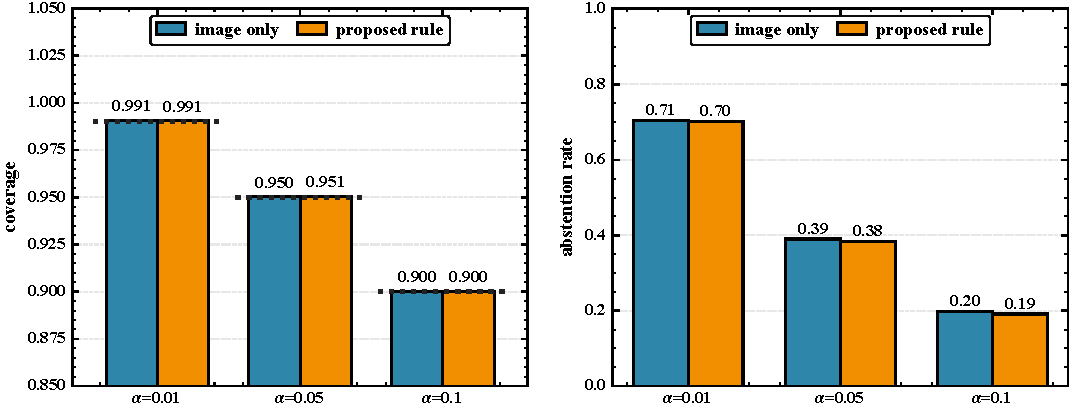
\includegraphics[width=\textwidth]{fus_conformal_synth_090}
\caption{Mondrian split-conformal abstention on a matched cohort at three target coverage levels. Top: empirical class-conditional coverage against the dotted target. Bottom: the fraction of women deferred to reach it.}
\label{fig:sconfsynth}
\end{figure}

\begin{figure}[!htbp]
\centering
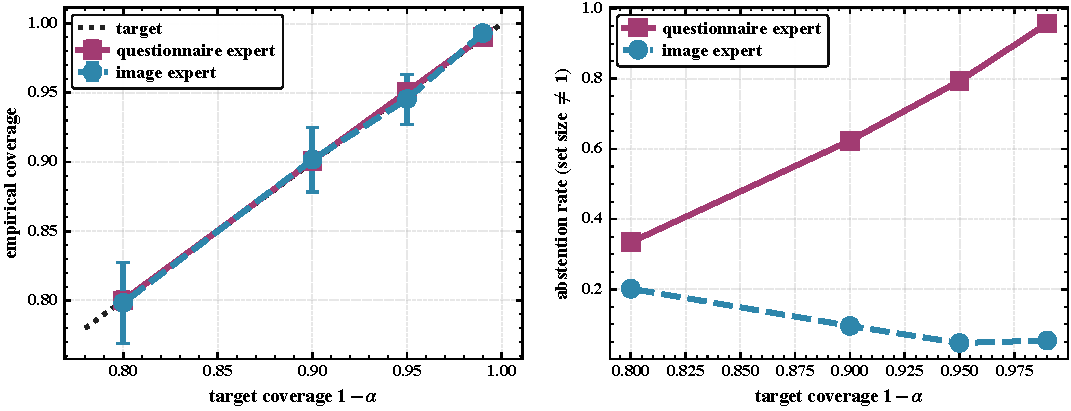
\includegraphics[width=\textwidth]{fus_conformal_real}
\caption{Conformal abstention applied to each expert individually on its own held-out data, before fusion. The questionnaire expert must defer far more often than the image expert to reach the same coverage, which is what a weak signal costs.}
\label{fig:sconfreal}
\end{figure}

\begin{table}[!htbp]
\caption{Conformal Coverage Under Deliberate Shift}
\label{tab:sconformal}
\centering\footnotesize
\begin{tabular}{@{}lcccc@{}}
\toprule
Scenario & Target & Coverage & SD & Deferral rate \\
\midrule
matched & 0.90 & 0.901 & 0.004 & 0.206 \\
dependence rho=0.6 & 0.90 & 0.880 & 0.003 & 0.195 \\
miscalibrated image & 0.90 & 0.911 & 0.004 & 0.481 \\
domain+prevalence shift & 0.90 & 0.755 & 0.006 & 0.301 \\
\bottomrule
\end{tabular}
\\[2pt]\begin{minipage}{\textwidth}\scriptsize Class-conditional coverage holds on matched data and fails under shift, because the guarantee is conditional on exchangeability between calibration and test data.\end{minipage}
\end{table}


\subsection{The price in paired data}
Table~\ref{tab:spaired} gives the numbers behind the paired-data figure in the main paper. A stacker trained on 50 paired women is worse than the unpaired rule by 0.014 AUROC; by 200 it is within 0.002, and it never overtakes the rule, remaining within 0.0004 even at 20,000 paired women. That is the expected result on matched cohorts, where the unpaired rule is already the Bayes rule, and it should not be read as an argument against collecting paired data: the value of paired data appears in Table~\ref{tab:sviolations}, where an oracle that can learn a residual dependence reaches 0.9217 at $\rho=0.6$ against 0.8847 for the rule.

\begin{table}[!htbp]
\caption{Stacker Minus Unpaired Rule, by Amount of Paired Data}
\label{tab:spaired}
\centering\footnotesize
\begin{tabular}{@{}lcc@{}}
\toprule
Paired patients & $\Delta$AUROC & SD \\
\midrule
50 & -0.0141 & 0.0391 \\
100 & -0.0043 & 0.0061 \\
200 & -0.0018 & 0.0017 \\
500 & -0.0018 & 0.0031 \\
1000 & -0.0018 & 0.0027 \\
5000 & -0.0002 & 0.0004 \\
20000 & -0.0004 & 0.0004 \\
\bottomrule
\end{tabular}
\\[2pt]\begin{minipage}{\textwidth}\scriptsize Negative values mean the stacker is worse than the rule that uses no paired data at all. It never overtakes it here, because on matched cohorts the rule is already optimal.\end{minipage}
\end{table}


\subsection{Net benefit}
Fig.~\ref{fig:sdecfus} gives the decision curve for the fused system on a matched synthetic cohort. Because that cohort is semi-synthetic, the curve describes the behaviour of the arithmetic under a stated generative model and is not evidence of clinical utility; we report it for completeness and would not cite it in support of deployment.

\begin{figure}[!htbp]
\centering
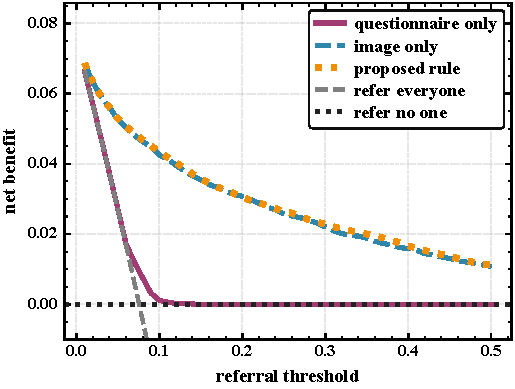
\includegraphics[width=3.45in]{fus_decision_090}
\caption{Decision-curve analysis on a matched synthetic cohort. A simulation result, not evidence of clinical utility.}
\label{fig:sdecfus}
\end{figure}

\end{document}
